\documentclass{article}


% if you need to pass options to natbib, use, e.g.:
%     \PassOptionsToPackage{numbers, compress}{natbib}
% before loading neurips_2023

% ready for submission
\usepackage[final]{neurips_2023}

% to avoid loading the natbib package, add option nonatbib:
%    \usepackage[nonatbib]{neurips_2023}


\usepackage[utf8]{inputenc} % allow utf-8 input
\usepackage[T1]{fontenc}    % use 8-bit T1 fonts
\usepackage{hyperref}       % hyperlinks
\usepackage{url}            % simple URL typesetting
\usepackage{booktabs}       % professional-quality tables
\usepackage{amsfonts}       % blackboard math symbols
\usepackage{nicefrac}       % compact symbols for 1/2, etc.
\usepackage{microtype}      % microtypography
\usepackage{xcolor}         % colors
\usepackage{graphicx}       % addtional package for show figures


\begin{document}


\maketitle

%%%%%%%Part 3 Audio Features Start%%%%%%%%%

\section{Audio Features}

\subsubsection{(a) Feature choice and dimension cut}
We checked the 13 frame features in each \texttt{.npz} file. Some were almost the same or did not add much information, for example \texttt{power} is almost equal to \texttt{energy}. We also dropped \texttt{mfcc\_delta2} and \texttt{flatness}. The nine groups we kept are in Table~\ref{tab:feat}.

We normalised every frame with a \texttt{StandardScaler}. Then we ran PCA. The first PCA keeps \textbf{95.4\%} of the variance with 62 components (Figure~\ref{fig:pca}). A second PCA cuts it to 50 dimensions.

\begin{table}[h]
    \caption{Retained frame feature groups (total $140$\,dims).}
    \label{tab:feat}
    \centering
    \begin{tabular}{lcl}
        \toprule
        Group & \#dims & Reason \\ \midrule
        Mel spectrogram            & 64 & dense spectral envelope \\
        MFCC + $\Delta$            & 64 & static \& dynamic timbre \\
        Spectral contrast          & 7  & noise vs. harmonic      \\
        Centroid, bandwidth, flux  & 3  & brightness / variation   \\
        Energy, ZCR                & 2  & loudness / noisiness     \\ \bottomrule
    \end{tabular}
\end{table}

\begin{figure}[h]
    \centering
    % PCA cumulative variance plot
    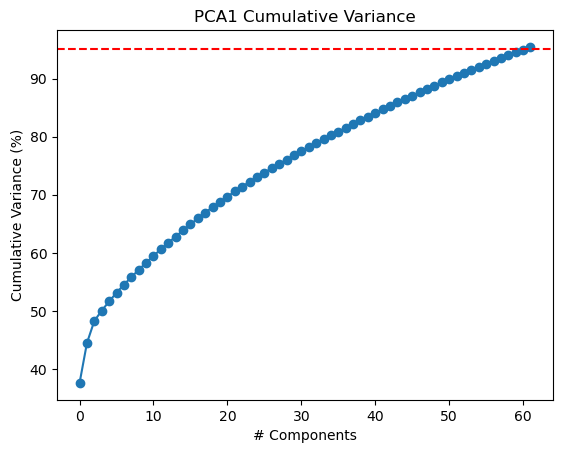
\includegraphics[width=.55\linewidth]{figs_tang/03_pca_cumulative_variance.png}
    \caption{Cumulative variance curve; the red dashed line marks 95\%.}
    \label{fig:pca}
\end{figure}

\subsubsection{(b) Fixed-length vectors for each region}
For every labelled segment $(t_\text{on}, t_\text{off})$ and the matching silent part, we make one 50‑D vector. We first project every frame through the two PCAs and then take the mean:
\[
\mathbf v = \frac{1}{N}\sum_{t=i_0}^{i_1-1}
\mathrm{PCA}_2(\mathrm{PCA}_1(\mathrm{Scaler}(\mathbf f_t))).
\]
This gives \textbf{51\,966} vectors: 35\,723 from events and 16\,243 from silence.

\subsubsection{(c) Clustering and silence check}
We tried $k$‑Means with $k=4\ldots30$. The best silhouette score (0.18) is at $k=4$ (Figure~\ref{fig:elbow}). Table~\ref{tab:cluster} shows the four clusters. Cluster~2 holds \textbf{84\%} of the silence vectors; most of the rest of the silence is in cluster~3.

\begin{figure}[h]
    \centering
    %Elbow+Silhouette plot
    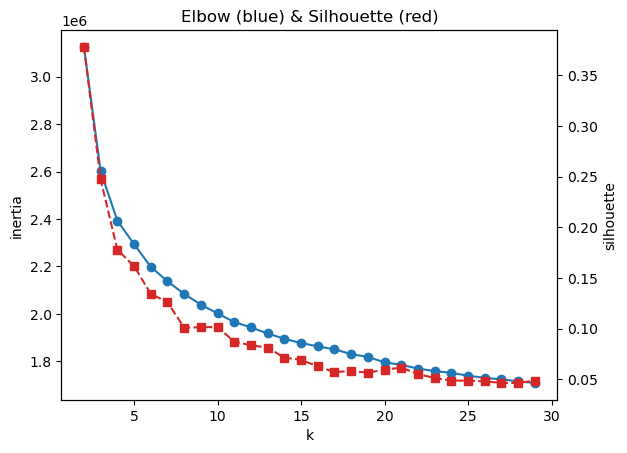
\includegraphics[width=.55\linewidth]{figs_tang/03_elbow_silhouette.png}
    \caption{Elbow curve (blue) and silhouette score (red) for different $k$.}
    \label{fig:elbow}
\end{figure}

\begin{table}[h]
    \caption{Cluster statistics for $k=4$.}
    \label{tab:cluster}
    \centering
    \begin{tabular}{cccc}
        \toprule
        id & size & silence (\%) & perceptual label \\ \midrule
        0 & 17\,944 & 19 & vehicle / rumble \\
        1 & 15\,745 & 11 & sharp metallic hits \\
        \textbf{2} & 6\,447 & \textbf{84} & near‑silence \\
        3 & 11\,830 & 47 & diffuse ambience \\ \bottomrule
    \end{tabular}
\end{table}

\begin{figure}[h]
    \centering
    % PCA scatter plots
    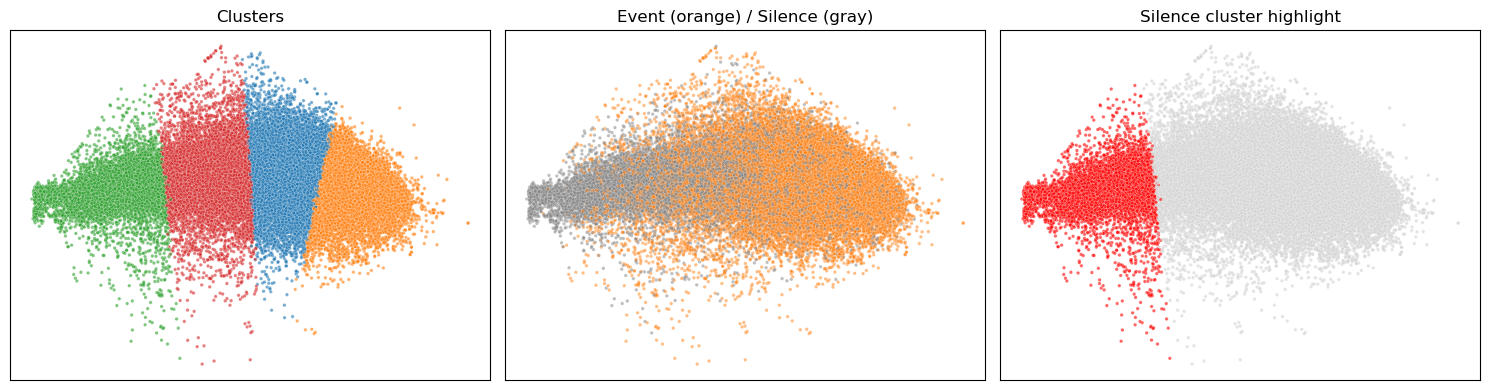
\includegraphics[width=.45\linewidth]{figs_tang/03_pca_clusters.png}
    \caption{Left: clusters in 2‑D PCA space; Right: event (orange) vs. silence (grey).}
    \label{fig:pca_scatter}
\end{figure}

These four clusters already split silence and three big sound types. They work as rough labels for training the detector later.

%%%%%%%Part 3 Audio Features Finish%%%%%%%%%


\end{document}